\apendice{Documentación técnica de programación}

\section{Introducción}
Este anexo contiene toda la información técnica de programación, incluyendo la estructura de directorios, las instalaciones necesarias, el proceso de arranque de la aplicación y los test generados. Esto es de gran utilidad para todo desarrollador/a que quiera realizar modificaciones al proyecto actual.
\section{Estructura de directorios}
\subsection{Estructura de directorios del \textit{frontend}}

\begin{itemize}
    \item \texttt{frontendAngular/}
    \begin{itemize}
        \item \texttt{.angular/} -- Archivos de configuración específica de Angular.
        \item \texttt{dist/} -- Archivos generados después de la construcción del proyecto.
        \item \texttt{node\_modules/} -- Dependencias de Node.js instaladas.
        \item \texttt{src/} -- Directorio principal de código fuente.
        \begin{itemize}
            \item \texttt{app/}
            \begin{itemize}
                \item \texttt{administracion/} -- Páginas específicas de la administración y su módulo.
                
                \item \texttt{aplicacion/} -- Páginas específicas de la administración y su módulo.
                \item \texttt{auth/} -- Módulo y componentes de autenticación.
                \item \texttt{prime-ng/} -- Configuración del módulo PrimeNG.
                \item \texttt{services/} -- Servicios que manejan la lógica de negocio y comunicación con la API.
                \item \texttt{shared/} -- Componentes compartidos en varios componentes.
                \item \texttt{app-routing.module.ts} -- Configuración de rutas de la aplicación.
                \item \texttt{app.component.css} -- Estilos del componente principal de la aplicación.
                \item \texttt{app.component.html} -- Plantilla HTML del componente principal.
                \item \texttt{app.component.ts} -- Lógica del componente principal.
                \item \texttt{app.module.ts} -- Módulo principal de la aplicación.
            \end{itemize}
            \item \texttt{assets/} -- Recursos estáticos de la aplicación (Imágenes).
            \begin{itemize}
                \item \texttt{.redirects} -- Configuración de redirecciones para Netlify.
                \item \texttt{index.html} -- Página principal de la aplicación.
                \item \texttt{main.ts} -- Punto de entrada principal de la aplicación.
                \item \texttt{styles.css} -- Estilos globales de la aplicación.
                \item \texttt{.editorconfig} -- Configuración del editor.
            \end{itemize}
        \end{itemize}
        \item \texttt{.gitignore} -- Archivos y directorios a ignorar por Git.
        \item \texttt{angular.json} -- Configuración del proyecto Angular.
        \item \texttt{package-lock.json} -- Descripción detallada de las dependencias instaladas.
        \item \texttt{package.json} -- Configuración y dependencias del proyecto.
        \item \texttt{README.md} -- Documentación del proyecto.
        \item \texttt{tsconfig.app.json} -- Configuración de TypeScript para la aplicación.
        \item \texttt{tsconfig.json} -- Configuración global de TypeScript.
        \item \texttt{tsconfig.spec.json} -- Configuración de TypeScript para pruebas.
    \end{itemize}
\end{itemize}


\subsection{Estructura de directorios del \textit{backend}}

\begin{itemize}
    \item \texttt{API PYTHON/}
    \begin{itemize}
        \item \texttt{app/} -- Directorio principal del código fuente de la aplicación.
        \begin{itemize}
            \item \texttt{Funciones\_Auxiliares/} -- Funciones auxiliares utilizadas en la aplicación.
            \begin{itemize}
                \item \texttt{automatizar\_correo.py} -- Script para automatizar el envío de correos.
                \item \texttt{funciones\_webscraping.py} -- Funciones para realizar web scraping.
            \end{itemize}
            \item \texttt{modelos/} -- Definición de modelos de datos.
            \begin{itemize}
                \item \texttt{\_\_init\_\_.py} -- Inicialización del paquete de modelos.
                \item \texttt{modelos.py} -- Definición de los modelos de la base de datos.
            \end{itemize}
            \item \texttt{modulos/} -- Módulos de la aplicación, organizados por funcionalidad.
            \begin{itemize}
                \item \texttt{botones/} -- Módulo con la funcionalidad de botones y permisos.
                \item \texttt{colaboradores/} -- Módulo con la gestión de colaboradores.
                \item \texttt{gestionEstimacion/} -- Módulo con la gestión de estimaciones.
                \item \texttt{gestionLibros/} -- Módulo con la gestión de libros.
                \item \texttt{importacionExportacion/} -- Módulo con la importación y exportación del catálogo.
                \item \texttt{roles/} -- Módulo con la gestión de roles de usuarios.
                \item \texttt{sugerencias/} -- Módulo con la gestión de sugerencias.
                \item \texttt{usuarios/} -- Módulo con la gestión de usuarios.
                \item \texttt{\_\_init\_\_.py} -- Inicialización del paquete de módulos.
            \end{itemize}
            \item \texttt{config.py} -- Archivo de configuración de la aplicación.
        \end{itemize}
        \item \texttt{instance/} -- Directorio de la base de datos local.
        \item \texttt{tests/} -- Directorio que contiene las pruebas unitarias.
        \item \texttt{requirements.txt} -- Archivo que lista las dependencias del proyecto.
        \item \texttt{run.py} -- Script para iniciar la aplicación.
    \end{itemize}
\end{itemize}

\section{Manual del programador}
Este manual tiene como objetivo formar a todo aquel que desee realizar desarrollos o modificaciones a este proyecto. En él se explican las instalaciones necesarias para generar el entorno de desarrollo, obtener el código, y una guía para ejecutarlo.

\subsection{Instalaciones necesarias}
Para este proyecto se requieren realizar las siguientes instalaciones:
\begin{itemize}
    \item Visual Studio Code
    \item Git
    \item NodeJS 20.11.1
    \item Python 3.12.1
\end{itemize}

\subsubsection{Visual Studio Code}
Este a sido el editor de código elegido para realizar este proyecto, por lo que es recomendable usarle por su facilidad de configuración y variedad de extensiones útiles.
Para instalar este editor de código debemos dirigirnos a la página oficial
\href{https://code.visualstudio.com/}{Visual Studio Code} y descargarnos la última versión estable.
\begin{figure}[h]
    \centering
    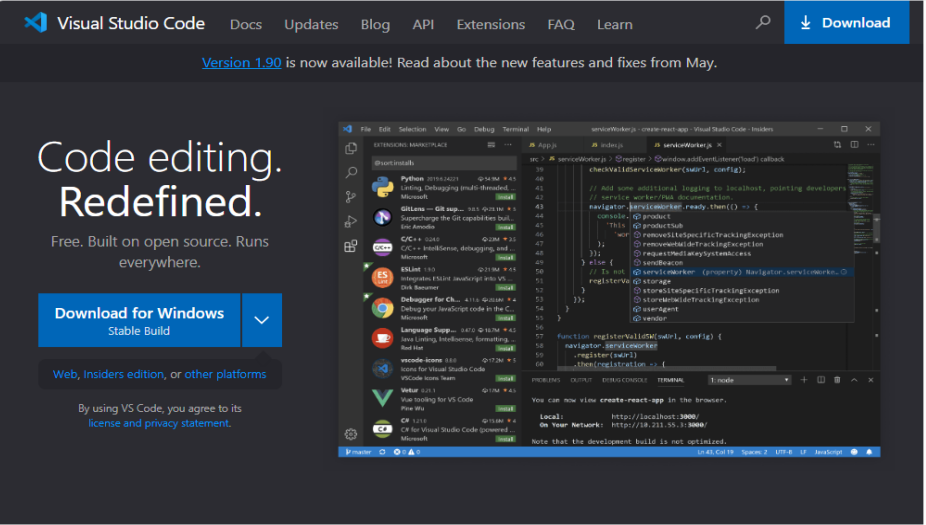
\includegraphics[width=0.75\linewidth]{Imagenes/VisualInstalacion.png}
    \caption{Página de instalación de Visual Studio Code}
    \label{Página de instalación de Visual Studio Code}
\end{figure}
\FloatBarrier


Una vez se nos descarga el instalador se mantienen las opciones por defecto y se procede a la instalación. Una vez instalado es recomendable dirigirse al apartado de extensiones e instalar las siguientes:
\begin{itemize}
    \item Angular Language Service
    \item Angular 17 Snippets
    \item Angular Schematics
    \item angular2-inline
    \item TypeScript Importer
    \item Python (Automáticamente instala las dos siguientes)
    \item Pylance
    \item Python Debugger
\end{itemize}

Además de esas, existen extensiones opcionales pero muy recomendables:
\begin{itemize}
    \item Error Lens
    \item Better Comments
    \item Material Icon Theme
    \item Auto Close Tag
    \item Activitus Bar
\end{itemize}

Si todos estos pasos se han realizado correctamente, deberíamos tener el Visual Studio iniciado correctamente y 13 extensiones instaladas.


\begin{figure}[h]
    \centering
    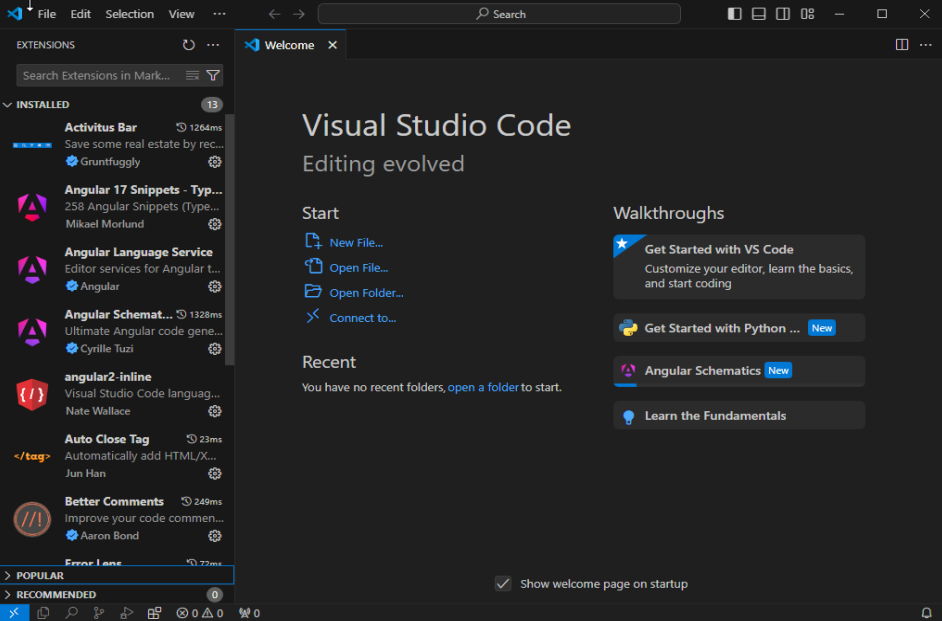
\includegraphics[width=0.75\linewidth]{Imagenes/ExtensionesVisual.png}
    \caption{Extensiones instaladas Visual Studio Code}
    \label{Extensiones instaladas Visual Studio Code}
\end{figure}
\FloatBarrier

\subsubsection{Python}

Este lenguaje es el usado para el \textit{backend} con la versión 3.12.1, por lo que para instalar esta versión debemos de dirigirnos a la web oficial de Python y seleccionar esa versión (\href{https://www.python.org/downloads/release/python-3121/}{Versión 3.12.1 de python}).
En la parte de abajo de esta página se encuentran todas las opciones de instalación, en este caso se va a escoger el instalador de Windows 64x ya que es el sistema operativo utilizado.
Una vez abierto el instalador, es recomendable activar la checkbox que agrega python.exe al PATH, ya que si no se encuentra activo puede acarrear problemas en el futuro.
Una vez seleccionamos esa opción, pulsamos en instalar ahora para que proceda con la instalación.

\begin{figure}[h]
    \centering
    \includegraphics[width=0.75\linewidth]{Imagenes/InstalaciónPython.png}
    \caption{Instalador de Python}
    \label{Instalador de Python}
\end{figure}
\FloatBarrier

\subsubsection{NodeJS}
NodeJS es el encargado de compilar el lenguaje TypeScript utilizado en Angular así como el administrados de dependencias del proyecto en la parte \textit{frontend}. En Prehistoria en Igualdad se ha utilizado la versión 20.11.1, la cual se instala desde esta URL \href{https://nodejs.org/en/blog/release/v20.11.1}{Versión 20.11.1 de node}

Ya dentro de la web de NodeJS bajamos en la página y encontramos la zona de instaladores. En este caso se instala la versión de Windows 64 bit en formato instalador.

Una vez abierto el instalador, se va dando al botón de siguiente aceptando las condiciones y el resto de campos se dejan por defecto.
Si tras la instalación, no sale en el instalador que se ha instalado correctamente, no es necesario realizar más pasos.

\begin{figure}[h]
    \centering
    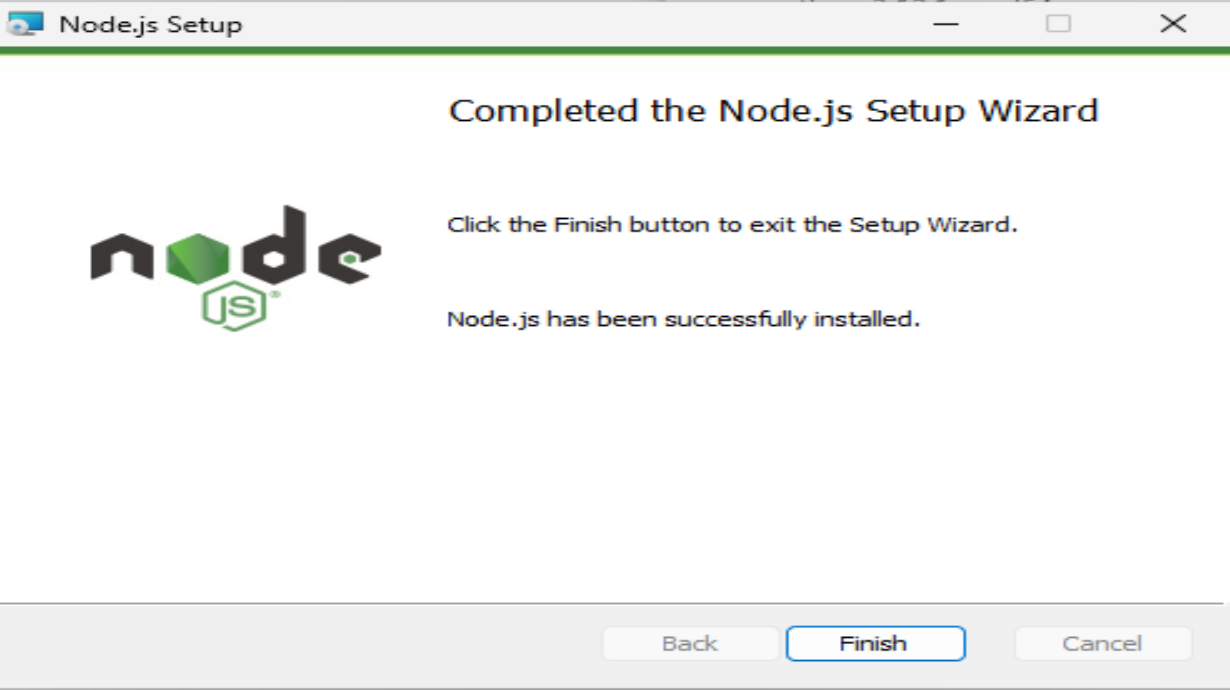
\includegraphics[width=0.75\linewidth]{Imagenes/InstaladorNode.png}
    \caption{Instalación existosa de NodeJS}
    \label{Instalación existosa de NodeJS}
\end{figure}
\FloatBarrier

\subsubsection{Git}
Git es una herramienta de control de versiones que se ha utilizado en este proyecto para ir actualizando los cambios en GitHub y que en este manual se va a utilizar para obtener el proyecto del repositorio para poder ejecutarlo desde local.
La instalación de Git comienza en la \href{https://www.git-scm.com/downloads}{página oficial}, donde descargaremos su instalador con la versión más reciente en la versión \textit{Standalone}.

Una vez descargado el instalador, nos pedirá por permisos de administración el poder realizar cambios. Una vez aceptado, se dejan todas las opciones por defecto y se da al botón de continuar para que se ejecute la instalación.

Si se ha instalado correctamente, al cerrar el instalador nos dará la opción de ver las últimas modificaciones de esta versión.


\subsection{Obtención del código fuente y Ejecución del código}
Para obtener el código del proyecto existen varias vías, pero en este caso se va a utilizar la herramienta ya instalada Git.

Con los comandos que se muestran a continuación se podrá descargar de manera rápida todos los ficheros.
\begin{itemize}
    \item Abrimos una terminal de Git en el directorio en el que queramos guardar el proyecto.
    \begin{figure}[h]
        \centering
        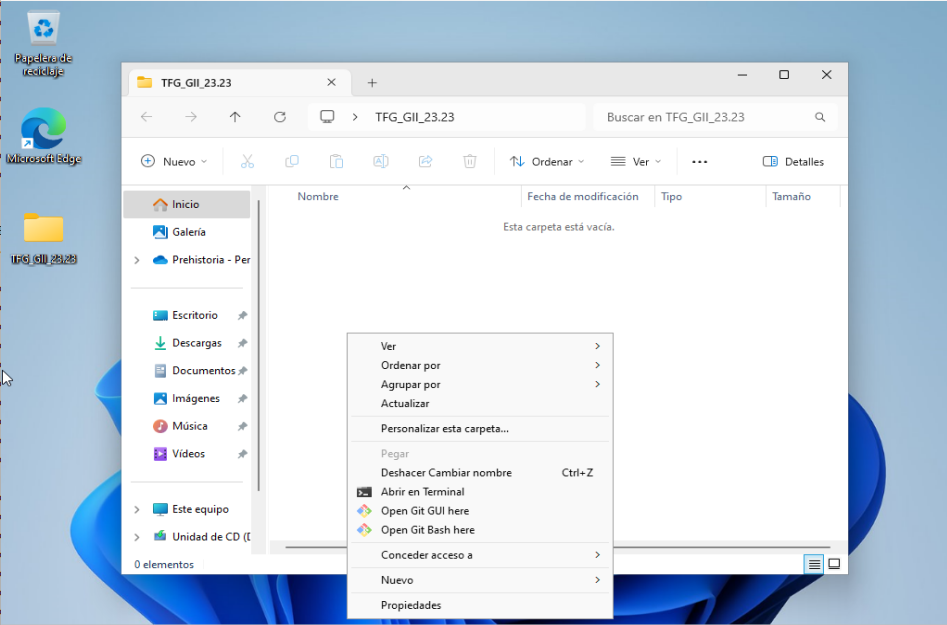
\includegraphics[width=0.75\linewidth]{Imagenes/AperturaTerminalGit.png}
        \caption{Apertura de terminal Git}
        \label{Apertura de terminal Git}
    \end{figure}
    \FloatBarrier
    \item Introducimos los siguientes comandos con la información personal:
    \begin{enumerate}
        \item git config --global user.name "Tu Nombre"
        \item git config --global user.email "tuemail@example.com"
    \end{enumerate}

    \begin{figure}[h]
        \centering
    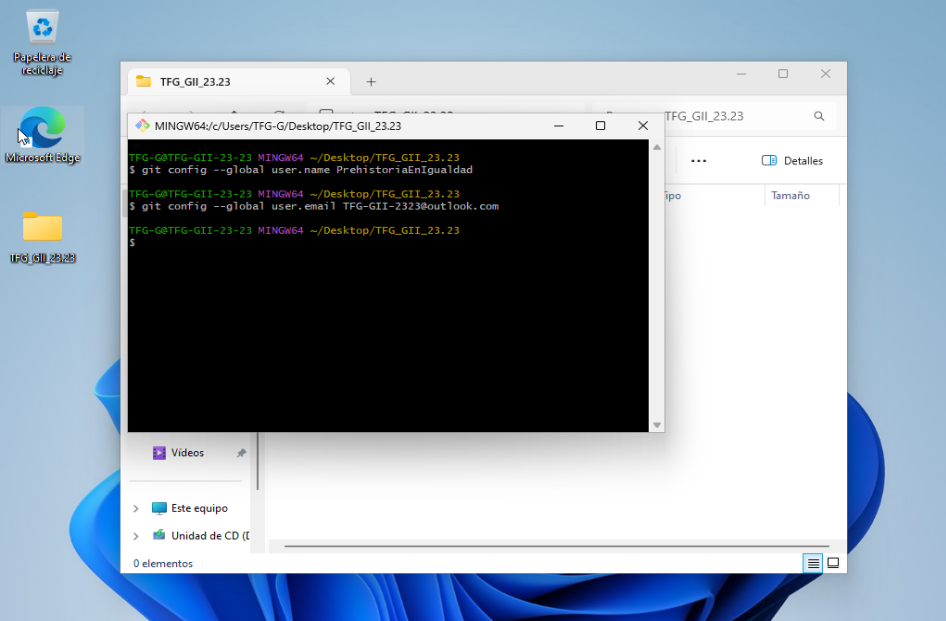
\includegraphics[width=1\linewidth]{Imagenes/ComandosUsuarioCorreoGit.png}
        \caption{Comandos de Usuario y correo de Git}
        \label{Comandos de Usuario y correo de Git}
    \end{figure}
    \FloatBarrier
    \item Ejecutamos el comando que clona el repositorio en local.
    \begin{enumerate}
        \item git clone https://github.com/DanielFernandezFdez/TFG\_GII\_23.23.git
    \end{enumerate}

    \begin{figure}[h]
        \centering
        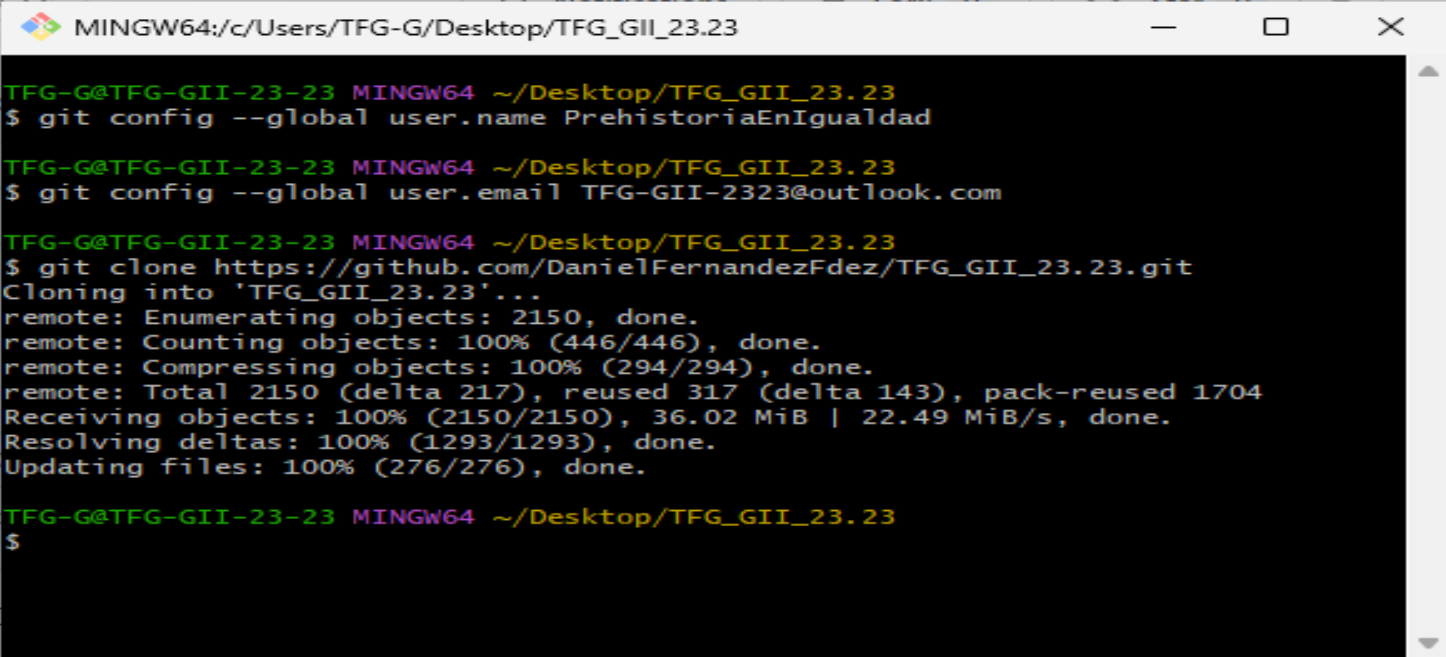
\includegraphics[width=0.75\linewidth]{Imagenes/GitClone.png}
        \caption{Clonación del repositorio}
        \label{Clonación del repositorio}
    \end{figure}
    \FloatBarrier
\end{itemize}


Una vez importado correctamente, desde visual le damos a abrir carpeta y seleccionamos el proyecto que acabamos de obtener.

Antes de comenzar con la ejecución, han de realizarse unos pasos previos para finalizar la instalación de dependencias.

\begin{itemize}
    \item Instalación de dependencias del \textit{backend}
    \begin{enumerate}
        \item Dentro de la carpeta 'API PYTHON' ejecutar el siguiente comando para generar un entorno virtual:

        python -m venv [Nombre del entorno]
        
        Si es satisfactoria la creación, dentro de la carpeta API PYTHON se generará una carpeta con el nombre dado.

        \item Activamos el entorno virtual para cargar las dependencias:

        [Nombre del entorno virtual]\textbackslash{Scripts}\textbackslash{Activate}

        Si se ha ejecutado correctamente nos tendría que aparecer el nombre en la línea de comandos entre paréntesis. En el caso de la figura \ref{Activar entorno virtual} se puede observar en la parte izquierda en color verde el nombre \texttt{EntornoVirtual}.

        \begin{figure}[h]
            \centering
            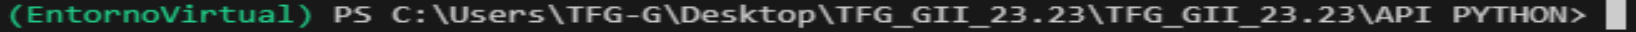
\includegraphics[width=1\linewidth]{Imagenes/ActivarVenv.png}
            \caption{Activar entorno virtual}
            \label{Activar entorno virtual}
        \end{figure}
        \FloatBarrier
        
        \item Con el entorno virtual activo volcamos las dependencias del archivo requirements.txt con el comando:

        py -m pip install -r requirements.txt

        \item Con todos estos pasos realizados, con ejecutar el comando \textit{python run.py} se iniciaría el backend. Es importante recordar que hay que activar el entorno virtual antes de iniciar la API.
    \end{enumerate}

    \item Instalación de dependencias del \textit{frontend}
    \begin{enumerate}
        \item Situarnos en la carpeta frontendAngular con la consola.
        \item Ejecutar el comando \textit{npm install} para instalar las dependencias y el \textit{framework} Angular.
        \item Una vez terminada la descarga, podemos arrancar el frontend con el comando \textit{npm start}
    \end{enumerate}
\end{itemize}

\subsubsection{Cambiar la configuración de producción a local}
\begin{itemize}
    \item En la parte del \textit{backend}, en el fichero config.py cambiar la variable db\_path a la comentada.

    \item En la parte del \textit{frontend}, en los ficheros service, cambiar la variable apiURL a la comentada.
\end{itemize}

\section{Pruebas del sistema}
En esta última sección se describen las pruebas disponibles para comprobar si los cambios han generado resultados inesperados, y así poder solucionarlos antes de realizar el despliegue.

\subsection{Ejecutar}
\begin{enumerate}
    \item Abre una terminal o línea de comandos en el Visual Studio Code.
    \item Navega al directorio de la carpeta \texttt{tests}.
    \item Ejecuta el siguiente comando para ejecutar todas las pruebas unitarias:

    pytest [nombre del test]

    Este comando ejecutará todas las pruebas definidas en el archivo y generará un reporte con los resultados.
    Si se pone simplemente \textit{pytest ./} y ejecutará todos los test de la carpeta.

\end{enumerate}

\subsubsection{Resultados de las Pruebas}
Después de ejecutar las pruebas, \texttt{pytest} generará un reporte en la terminal mostrando qué pruebas pasaron y cuáles fallaron. Si alguna prueba falla, \texttt{pytest} proporcionará detalles sobre la causa del fallo, permitiéndote identificar y corregir el problema.

\subsection{Pruebas Manuales con Postman}

Además de las pruebas unitarias, se recomienda realizar pruebas manuales utilizando Postman para verificar el comportamiento de las APIs del sistema. Postman es una herramienta potente para probar y documentar APIs. A continuación se describe cómo utilizar Postman para realizar estas pruebas.

\subsubsection{Configuración de Postman}
Si aún no tienes Postman instalado, puedes descargarlo e instalarlo desde \href{https://www.postman.com/downloads/}{Postman}. Una vez instalado, sigue estos pasos:

\begin{enumerate}
    \item Abrir Postman.
    \item Agregar una nueva solicitud a la búsqueda con la URL local. Configurar el tipo de solicitud (GET, POST, PUT, DELETE).
    \item Configurar los parámetros necesarios, como headers y cuerpo en formato JSON.
    \item Envíar la solicitud y verificar la respuesta. Postman mostrará el código de estado HTTP y el cuerpo de la respuesta recibida del servidor.
\end{enumerate}

\subsubsection{Validación de Respuestas}
Para cada solicitud, hay que asegurarse que la respuesta recibida es la esperada. Esto incluye verificar:
\begin{itemize}
    \item El código de estado HTTP (por ejemplo, 200 OK, 404 Not Found, 500 Internal Server Error).
    \item El contenido del cuerpo de la respuesta, asegurando que los datos devueltos sean correctos y estén en el formato esperado.
    \item Los headers de la respuesta, si es necesario.
\end{itemize}
